\chapter{Protección frente a contactos directos e indirectos}
\section{Riesgos de la utilización de la electricidad}
\begin{itemize}
	\item Deterioro aislamiento, incendio, explosión, etc.
	\begin{itemize}
		\item Cortocircuitos
		\item Sobrecargas
		\item Sobretensiones
		\item Subtensiones
		\item Desequilibrios
	\end{itemize}
	\item Riesgo para las personas
	\begin{itemize}
		\item Choque eléctrico
		\begin{itemize}
			\item Contacto Directo: entre partes activas y/o tierra
			\item Contacto Indirecto: entre masas bajo tensión y tierra
		\end{itemize}
		\item Quemaduras por efectos térmicos
	\end{itemize}
\end{itemize}
\section{Efectos biológicos de la corriente eléctrica}
\subsection{Intensidad de la corriente}
Depende de:
\begin{itemize}
	\item La tensión de contacto
	\item Superficie de contacto
	\item Condiciones en el contacto: humedad, presión,
	temperatura y materiales interpuestos
	\item Frecuencia de la señal
\end{itemize}

El mayor riesgo en función de la corriente existe a la frecuencia de red $\approx 50 Hz$ con un umbral de no soltar de $\approx 10 mA$ mientras que a frecuencias altas $\approx 8 kHz$ o en DC el umbral de no soltar es de $\approx 50 mA$.
\newline

Para obtener el modelo es necesario obtener la impedancia del cuerpo humano que depende de muchos factores como la tensión de contacto, la superficie o la humedad del entorno. No obstante, se puede tomar un valor máximo de esta impedancia de $Z=1050\Omega$ 
\newpage
\subsection{Tiempo de contacto}
Cuanto más tiempo de contacto más grave es una corriente, se recoge mediante la siguiente gráfica:
\begin{figure}[H]
	\centering
	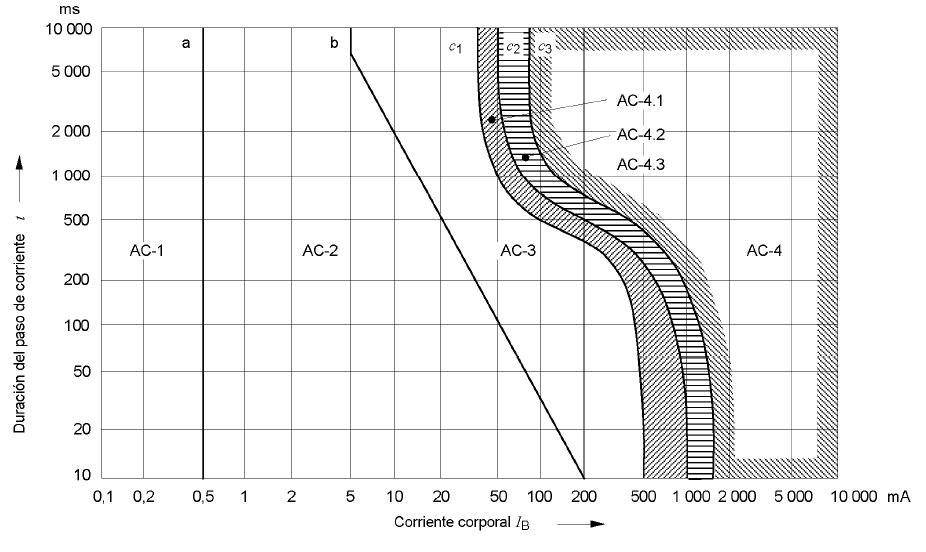
\includegraphics[width=0.7\linewidth]{Images/23}
	\caption{Zonas tiempo
		corriente convencionales de los efectos de corrientes alternas (15
		Hz 100 Hz) sobre personas para una trayectoria mano izquierda a pies}
	\label{fig:23}
\end{figure}

En esta gráfica existen las siguientes zonas:
\begin{itemize}
	\item \textbf{AC-1}: Efectos no perceptibles
	\item \textbf{AC-2}: Ningún efecto perjudicial
	\item \textbf{AC-3}: Habitualmente sin daños orgánicos
	\item \textbf{AC-4.1}: 5\% de riesgo de fibrilación cardíaca
	\item \textbf{AC-4.2}: 50\% de riesgo de fibrilación cardíaca
	\item \textbf{AC-4.3}: >50\% de riesgo de fibrilación cardíaca
	\item \textbf{AC-4}: 100\% de riesgo de fibrilación cardíaca
\end{itemize}

Aunque los problemas biológicos derivados de fenómenos eléctricos dependen de la corriente, existe una curva equivalente para tensiones de contacto (no recogida en la normativa) para local conductor $U_{L2}$ y no conductor $U_{L1}$.
\begin{figure}[H]
	\centering
	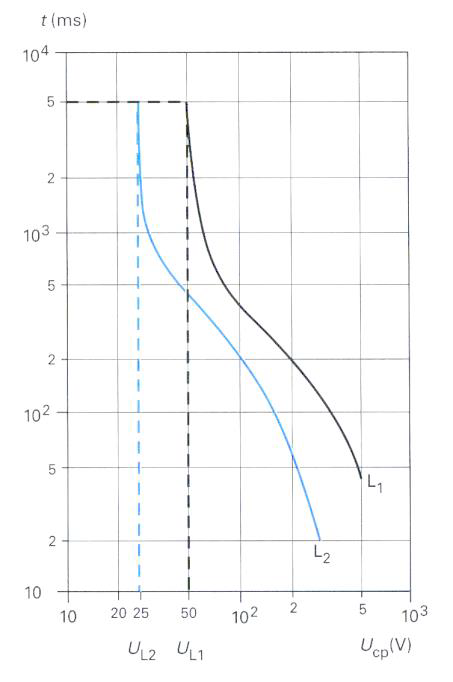
\includegraphics[width=0.4\linewidth]{Images/24}
	\label{fig:24}
\end{figure}

\subsection{Trayectoria por el cuerpo humano}
Se emplea un factor de corriente del corazón, F:
\begin{figure}[H]
	\centering
	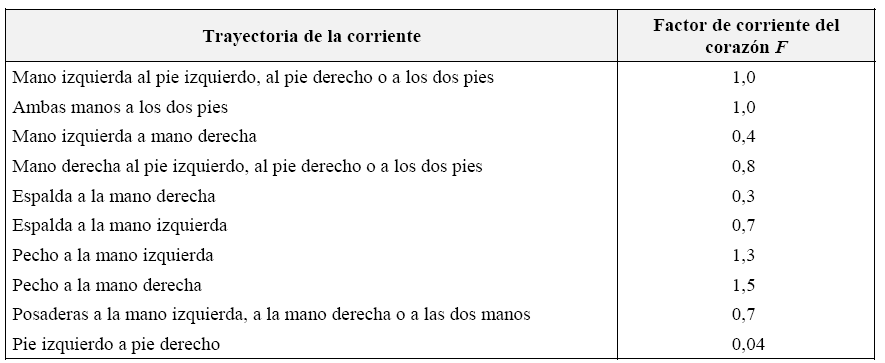
\includegraphics[width=0.7\linewidth]{Images/25}
	\label{fig:25}
\end{figure}

\begin{equation}
	I_{medida}=\dfrac{I_{\text{mano izquierda-pies}}}{F}
\end{equation}
\section{Métodos de protección frente a contactos directos}
\begin{itemize}
	\item Protección completa
	\begin{itemize}
		\item Aislamiento de las partes activas: viene recogida en los distintos ITC-BT en función del tipo de red
		
		\item Barreras o envolventes: se emplean los índices de protección IP
		\begin{enumerate}
			\item Primera cifra
			Protección contra
			cuerpos sólidos (cifras 0 a 6, o letra x) $\rightarrow$ 0 sin protección y 6 totalmente protegido contra el polvo.
			\item Segunda cifra
			Protección contra
			cuerpos líquidos (cifras 0 a 8, o letra x) $\rightarrow$ 0 sin protección y 8 totalmente protegido contra los efectos prolongados de la inmersión bajo presión.
			\item Letra adicional (opcional): Protección contra el acceso a partes peligrosas con
			\begin{enumerate}
				\item A: dorso de la mano
				\item B: dedo
				\item C: herramienta
				\item D: alambre
			\end{enumerate}
			\item Letra suplementaria (opcional)
			\begin{enumerate}
				\item H: material de alta tensión 
				\item V: movimiento durante el ensayo de agua
				\item S: inmóvil durante el ensayo de agua
				\item W: intemperie
			\end{enumerate}
		\end{enumerate}

		\item Utilización de muy baja tensión de seguridad: constituye una protección contra contactos directos e indirectos. Se alimenta mediante un transformador de aislamiento de seguridad con resistencia de aislamiento $R\ge 0.25M\Omega$, conductores separados de otros circuitos y masas no conectadas al conductor de protección o tierra.
		\begin{itemize}
			\item Local seco
			\begin{itemize}
				\item AC: 50V
				\item DC: 75V
			\end{itemize} 
			\item Piscina
			\begin{itemize}
				\item AC: 12V
				\item DC: 30V
			\end{itemize} 
		\end{itemize}
	\end{itemize}
	\item Protección parcial: solo se debería usar en locales accesibles solo a personal autorizado y se emplea para evitar contactos no intencionados con las partes activas
	\begin{itemize}
		\item Protección por medio de obstáculos
		\item Fuera de alcance por alejamiento
	\end{itemize}
	\item Protección suplementaria: \textbf{solo esta destinada a complementar otras medidas de protección contra contacto directo}. Sensibilidad, $\Delta I_n\le 30 mA$.
	Cuando las corrientes diferenciales puedan ser no senoidales
	deben utilizarse diferenciales de, al menos, clase A
\end{itemize}
\section{Métodos de protección frente a contactos indirectos}
Medidas de protección a utilizar:
\begin{itemize}
	\item Corte automático de la alimentación: es obligatorio cuando a causa de un defecto puede producirse un efecto peligroso. Puede darse en las siguientes condiciones:
	\begin{itemize}
		\item Existencia de “bucle de defecto” que permite la circulación de la corriente de
		defecto.
		\begin{itemize}
			\item El bucle de defecto depende de conexión a tierra: TT, TN ó IT
			\item  Implica conexión equipotencial según ITC BT 18 y ITC BT 19
		\end{itemize}
		\item Selección del dispositivo de desconexión según esquema de conexión a tierra
		que abra la corriente de defecto en un tiempo adecuado según ITC BT 24
		\begin{itemize}
			\item Esquema TT: Interruptores diferenciales
			\item Esquema IT: Interruptores automáticos
			\item Esquema TN: Interruptores automáticos
		\end{itemize}
		\item Tensión
		límite convencional en corriente alterna
		\begin{itemize}
			\item Locales no conductores o locales secos: 50 V
			\item Locales conductores o húmedos o mojados: 24 V
			\item Instalaciones subacuáticas: Piscinas y fuentes: 12 V (ITC
		\end{itemize}
	\end{itemize}
	\item Empleo de equipos de clase II o aislamiento equivalente: 
	\begin{itemize}
		\item Definición de aislamiento clase II en Norma UNE EN 60439-1
		\item Es un aislamiento doble o reforzado, se denomina: “aislamiento total”
		\item La mayor parte de los receptores portátiles o semimóviles , están
		provistos de doble aislamiento
		\item
		Las partes conductoras existentes no deben conectarse a un conductor
		de protección
		\item
		Si es necesario que conductores de protección pasen a través de la
		envolvente deben aislarse como partes activas
		\item
		En la GUIA-BT-24 se indican las condiciones que deben cumplir las
		canalizaciones y cables para que se consideren con aislamiento doble o
		reforzado
	\end{itemize}
\end{itemize}

Métodos de protección a utilizar en instalaciones supervisadas:
\begin{itemize}
	\item Protección en locales o emplazamientos no conductores
	(paredes aislantes, alejamiento o interposición de obstáculos entre
	masas y elementos conductores): 
	\begin{itemize}
		\item Para tensión nominal $U\le 500V \rightarrow R \ge50k\Omega$
		\item Para tensión nominal $U> 500V \rightarrow R \ge 100k\Omega$
	\end{itemize}
	\item Protección mediante conexiones equipotenciales locales no
	conectadas a tierra
	\item Protección por separación eléctrica (masas no conectadas a
	tierra)
\end{itemize}